\documentclass[12pt,a4paper]{article}
%%%%%%%%%%%%%%%%%%%%导言区%%%%%%%%%%%%%%%
\usepackage[BoldFont,SlantFont]{xeCJK}
\usepackage[dvips]{graphicx}
\setCJKmainfont[BoldFont=SimSun,ItalicFont=SimSun]{SimSun}
\setmainfont{Times New Roman}
\addtolength{\hoffset}{-1cm}
\addtolength{\voffset}{-2cm}
\addtolength{\textheight}{4cm}
\addtolength{\textwidth}{2cm}
\title{NIOS II Linux Tutorial}
\author{BearChen \and Annxl}
%%%%%%%%%%%%%%%%%%%%正文%%%%%%%%%%%%%%%
\begin{document}
\maketitle{}
\newpage{}
%%%%%%%%%%%%%%%%%%%%前言%%%%%%%%%%%%%%%
\section{前言}
本文由\textbf{texlive 2010}构建.

这是一个\textbf{NIOS II Linux}开发的入门教程,拟包括以下几个部分:\footnote{随着编写计划的变化,可能会有增减.}
\begin{itemize}
\item 介绍\textbf{NIOS II Linux}开发环境;
\item 一个完整的流程;
\item 创建自己的SOPC系统和Linux内核;
\item linux下驱动开发举例;
\item linux下普通应用程序开发;
\item FTK应用程序开发;
\end{itemize}
%%%%%%%%%%%%%%%%%%%%构建开发环境%%%%%%%%%%%%%%%
\newpage{}
\section{构建开发环境}
2009年9月,nioswiki社区推出基于NIOS II处理器的linux内核开发包,为开发者提供一种新的系统方案,这个方案
有其特有的优势:
\begin{itemize}
\item \textit{sopc}的架构使得针对各种特定场合可以构建不同的片上系统,相比ASIC(专用芯片)方案灵活性要高出不少;
\item 社区提供的开发包针对Altera的外设IP提供驱动,同时提供大量应用函数库和应用程序;
\end{itemize}

当然,正是由于sopc的灵活性,使得自定义IP大量涌现,针对自定义IP的驱动编写任务被转移到每个独立的开发者身上,同时由于每个
开发者构建的SOPC中同一设备的\underline{名字,功能}不尽相同,如何才能使同一个内核开发包针对不同名字的同一种IP以及各种IP具有统一的管理能力
是一个令人头疼的问题.

使用\textbf{NIOS II Linux}开发需要搭建硬件和软件环境.目前已知的开发环境有两类:
\begin{table}[!hbtp]
\centering
\begin{tabular}{|l|p{0.68\textwidth}|}
\hline
完全在linux下开发 & 在linux下安装linux版本的Quartus II和NiosII IDE开发工具,同时安装nios-linux内核开发包.
据我所知目前只有\textbf{Ubuntu9.04}可以兼容,Ubuntu9.10及以上版本暂时不支持\footnote{不支持的原因是nios2-download脚本在Ubuntu9.10及
以上版本中部分无法执行.而官方推荐的Redhat企业版和Fedora等均可配置.};\\
\hline
Windows+Linux虚拟机 & 这种方案更适合大多数平时工作在Windows环境下的开发者.本文接下来将介绍这种方案的配置;\footnote{由于在linux下
的usb-blaster驱动比windows下性能要相对差些,当构建的系统选择以JTAG-UART作为终端时,在linux环境下的``nios2-terminal''命令会导致系统阻塞,此时
我更倾向于使用本方案.} \\
\hline
\end{tabular}
\end{table}
\subsection{硬件环境}
在Windows安装QuartusII和相应版本的NiosII IDE.写本文时使用的是当时的最高版本9.0.因此大于等于该版本都应该没有问题.这里不赘述安装过程.

安装完成后,通过QuartusII中的\fbox{SOPC Builder}生成带nios cpu的片上系统,通过QuartusII进行硬件编译,使用\fbox{nios shell command}生成
片上系统对应的内核头文件``custom\_fpga.h'',并通过shell进行硬件下载,内核下载,硬件和内核烧写等工作.图\ref{fshell}是Windows下shell的启动
图标\footnote{其实NIOS II Shell就是定制版的Cygwin,因此可运行部分linux命令,如cd,cp,rm等}.图\ref{fshellgui}为Shell运行界面\\
\begin{figure}[!htbc]
\centering
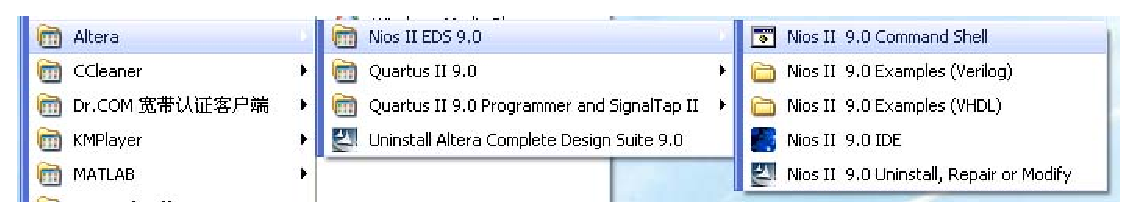
\includegraphics[width=1\textwidth]{pic/f_shell_icon.eps}
\caption{NIOS II Shell启动图标\label{fshell}}
\end{figure}
\begin{figure}[!htcb]
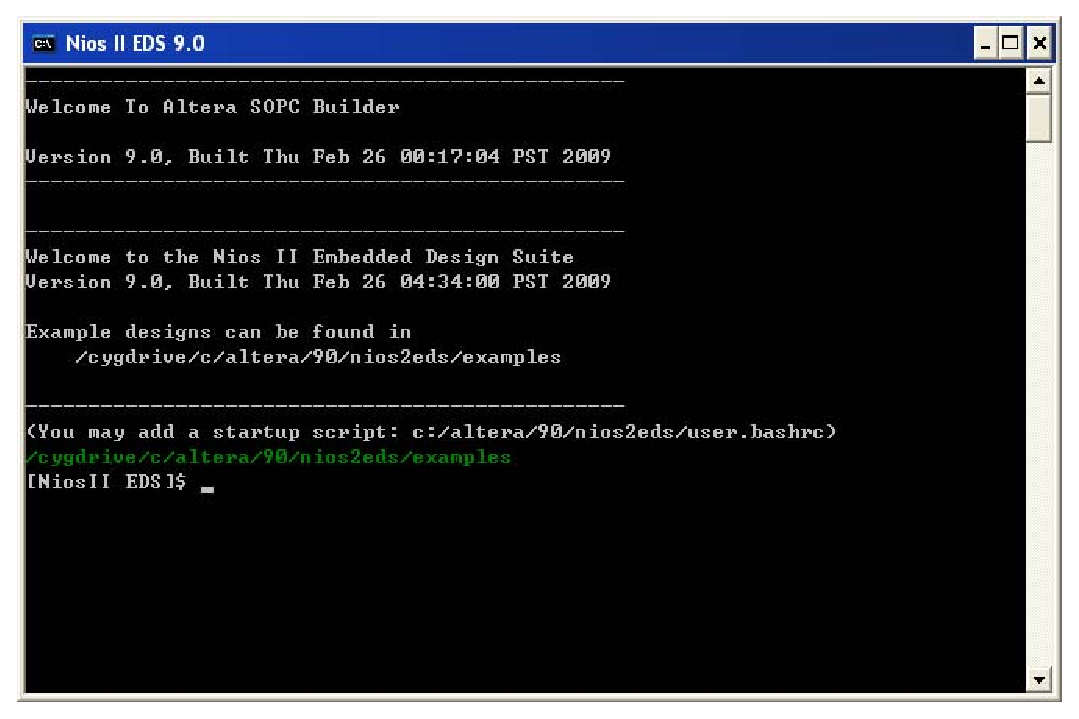
\includegraphics[width=1\textwidth]{pic/f_shell.eps}
\caption{NIOS II Shell运行界面\label{fshellgui}}
\end{figure}
\subsection{软件环境}
linux内核驱动和应用程序的开发都需要在类Unix操作系统下进行,最普遍的就是Linux操作系统.这里我们选择流行程度最高的Ubuntu操作系统作为开发平台.

首先我们要安装一款虚拟机软件\footnote{Windows下有Vmware,Virtual Box等}.通过该软件创建虚拟机并安装Ubuntu.安装好的虚拟机系统要满足两个要求:
\begin{itemize}
\item 能够连接互联网,下载内核开发所需的文件;
\item 能够与宿主机(Windows)交换文件.宿主机下生成的头文件要传入虚拟机中交给内核开发包使用,而虚拟机下生成的内核可执行文件要
在window下通过nios shell下载;
\end{itemize}

我们以Virtual Box为例说明如何操作.
\subsubsection{虚拟机安装Ubuntu并做相关设置}
创建虚拟机之前,本地电脑上需要有的东西包括:
\begin{itemize}
\item Ubuntu安装光盘或ISO镜像文件;
\item 已安装好Virtual Box软件;
\item 足够的硬盘空间(10G左右);
\end{itemize}

在Virtual Box主页面菜单上选择\fbox{控制-->新建},操作系统类型选择\textbf{Linux},版本选择\textbf{Ubuntu},如图\ref{f_create_vb1}所示.
\begin{figure}[!bthp]
\centering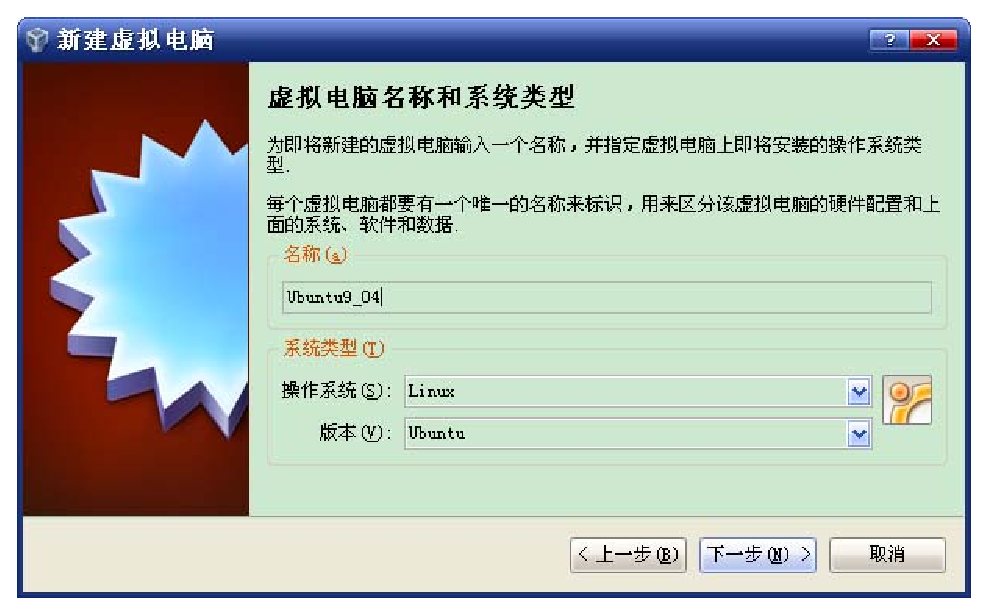
\includegraphics[width=1\textwidth]{pic/f_create_vb1.eps}
\caption{创建虚拟机:整体设定\label{f_create_vb1}}
\end{figure}
内存选择为当前系统内存一半略少,尽量发挥系统性能.硬盘选择"创建新的虚拟硬盘"并选择"固定大小"\footnote{相对于动态增长,
固定大小使得虚拟机运行速度更快}.硬盘创建完成后确定即可.
\begin{figure}[!bthp]
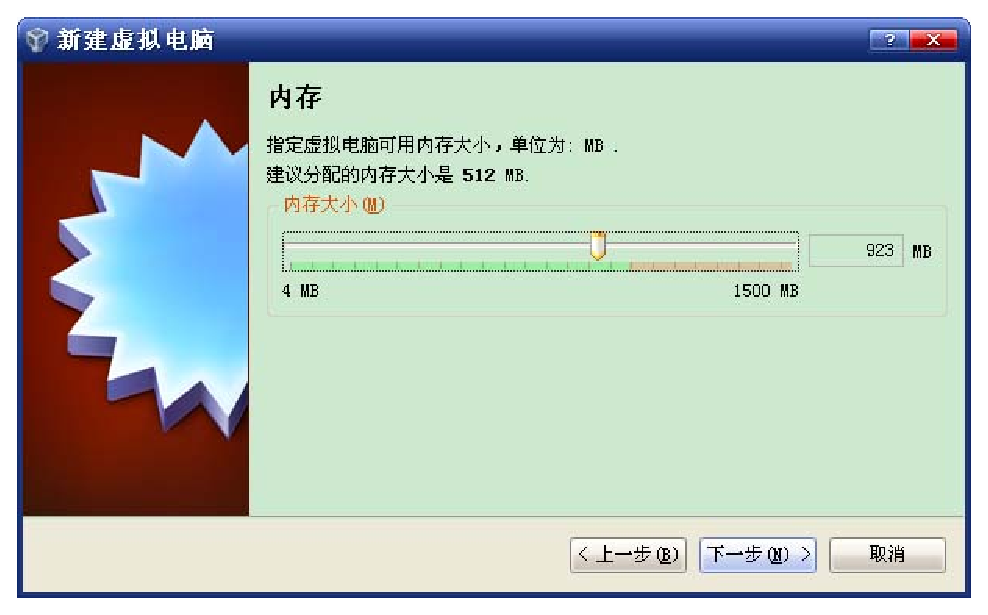
\includegraphics[width=1\textwidth]{pic/f_create_vb_mem.eps}
\caption{创建虚拟机:设置内存}
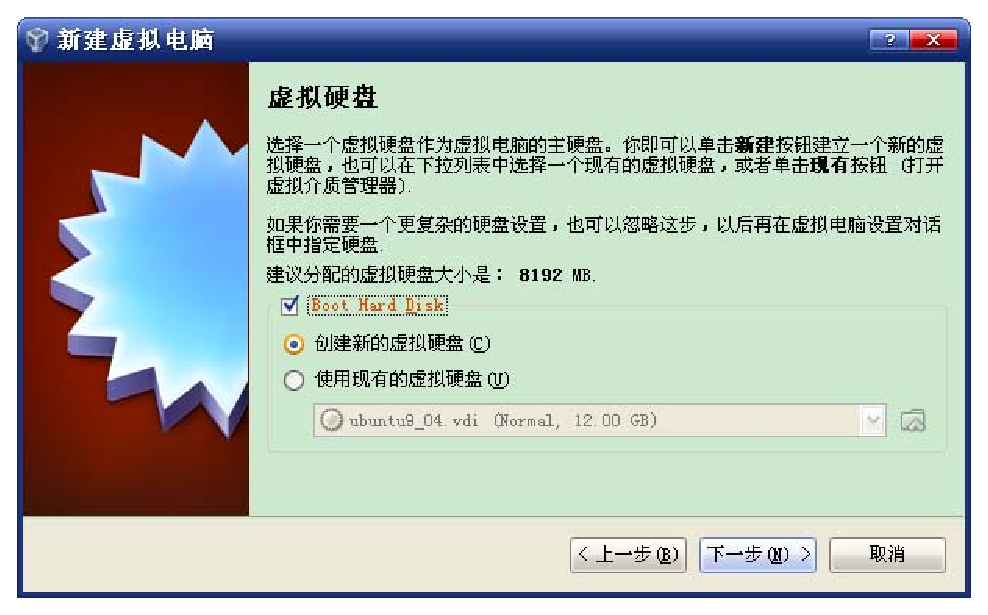
\includegraphics[width=1\textwidth]{pic/f_create_vb_hdisk.eps}
\caption{创建虚拟机:创建虚拟磁盘}
\end{figure}
\begin{figure}[!bthp]
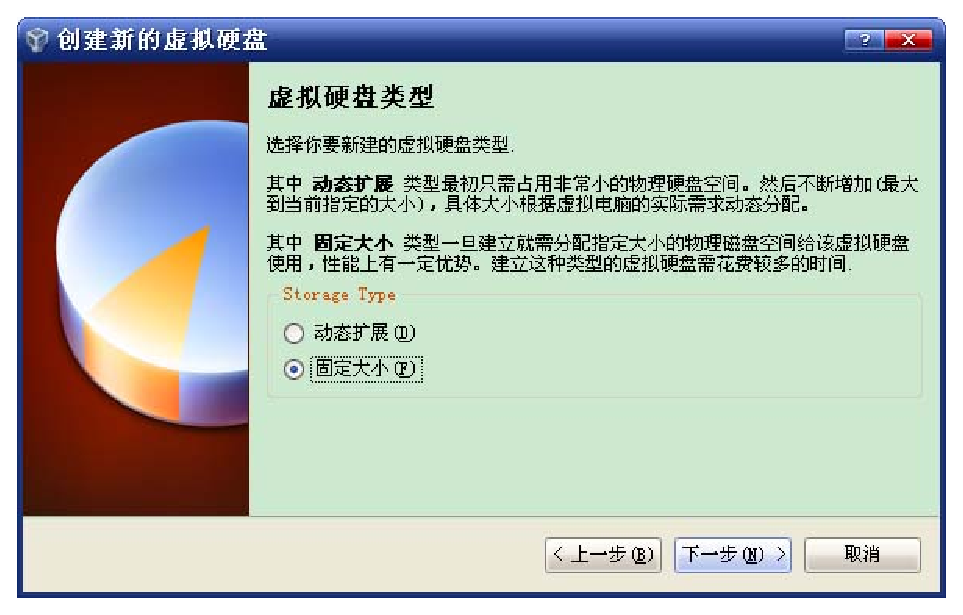
\includegraphics[width=1\textwidth]{pic/f_create_vb_hdisk1.eps}
\caption{创建虚拟机:创建虚拟磁盘}
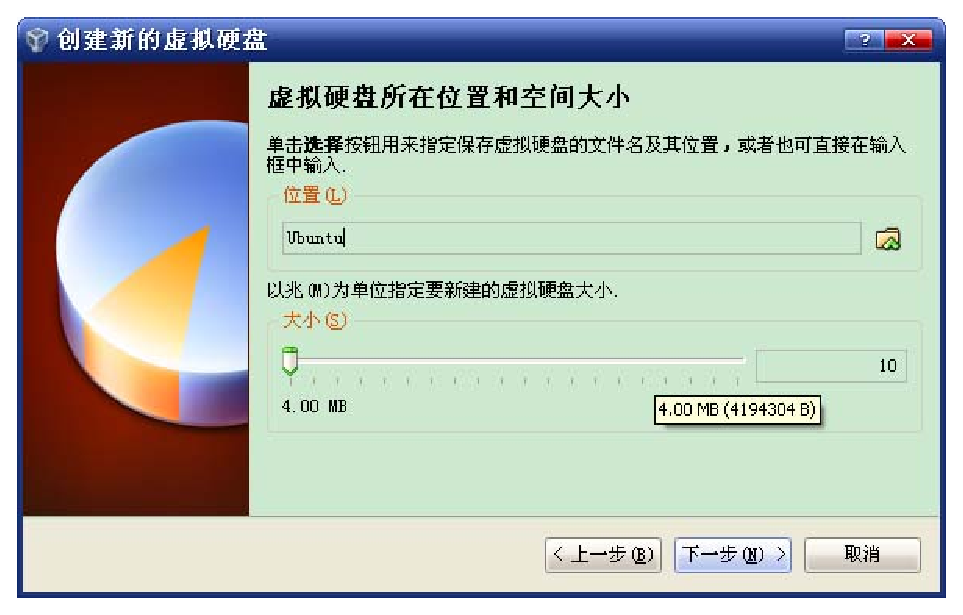
\includegraphics[width=1\textwidth]{pic/f_create_vb_hdisk2.eps}
\caption{创建虚拟机:创建虚拟磁盘}
\end{figure}
\newpage
到现在为止,虚拟机已经创建完毕.但是当前的虚拟机内没有任何系统,甚至连分区都没有,此时需要通过光驱安装操作系统.本文使用ISO镜像
文件进行安装.

在没有运行虚拟机的情况下,点击\fbox{设置}图标,右侧找到"介质"一栏,对ISO进行注册.如图\ref{iso0},\ref{iso1}和\ref{iso2}所示.
\begin{figure}[!bthp]
\centering
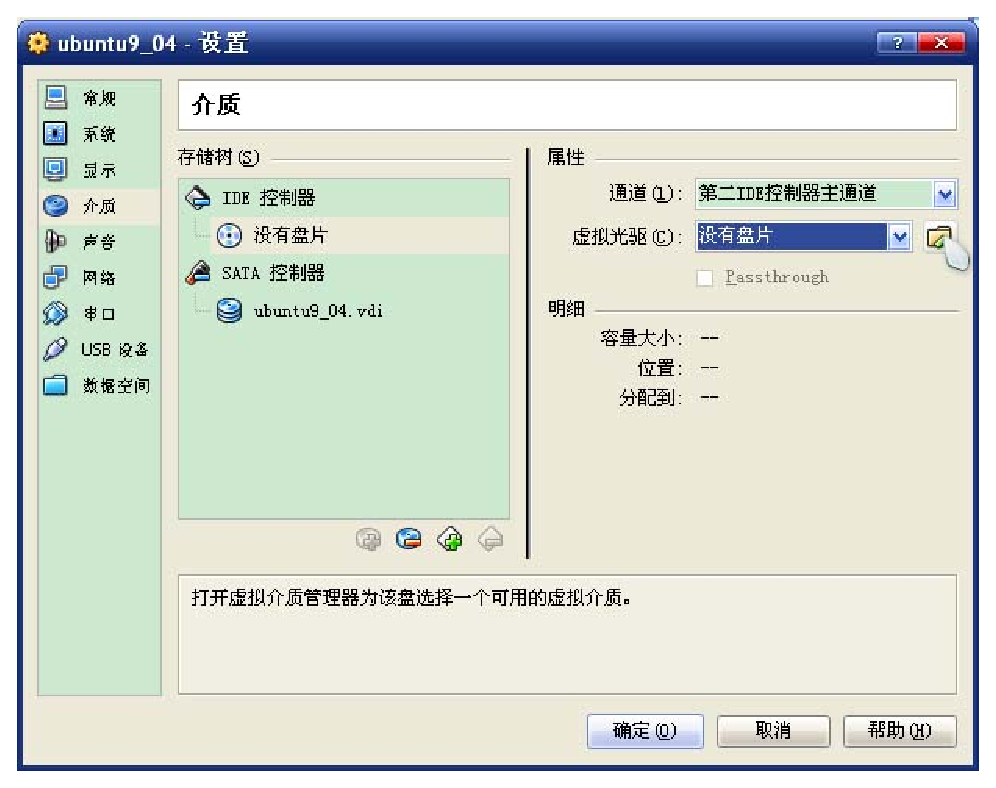
\includegraphics[width=0.8\textwidth,scale=0.8]{pic/f_vb_setting_iso.eps}
\caption{设置ISO\label{iso0}}
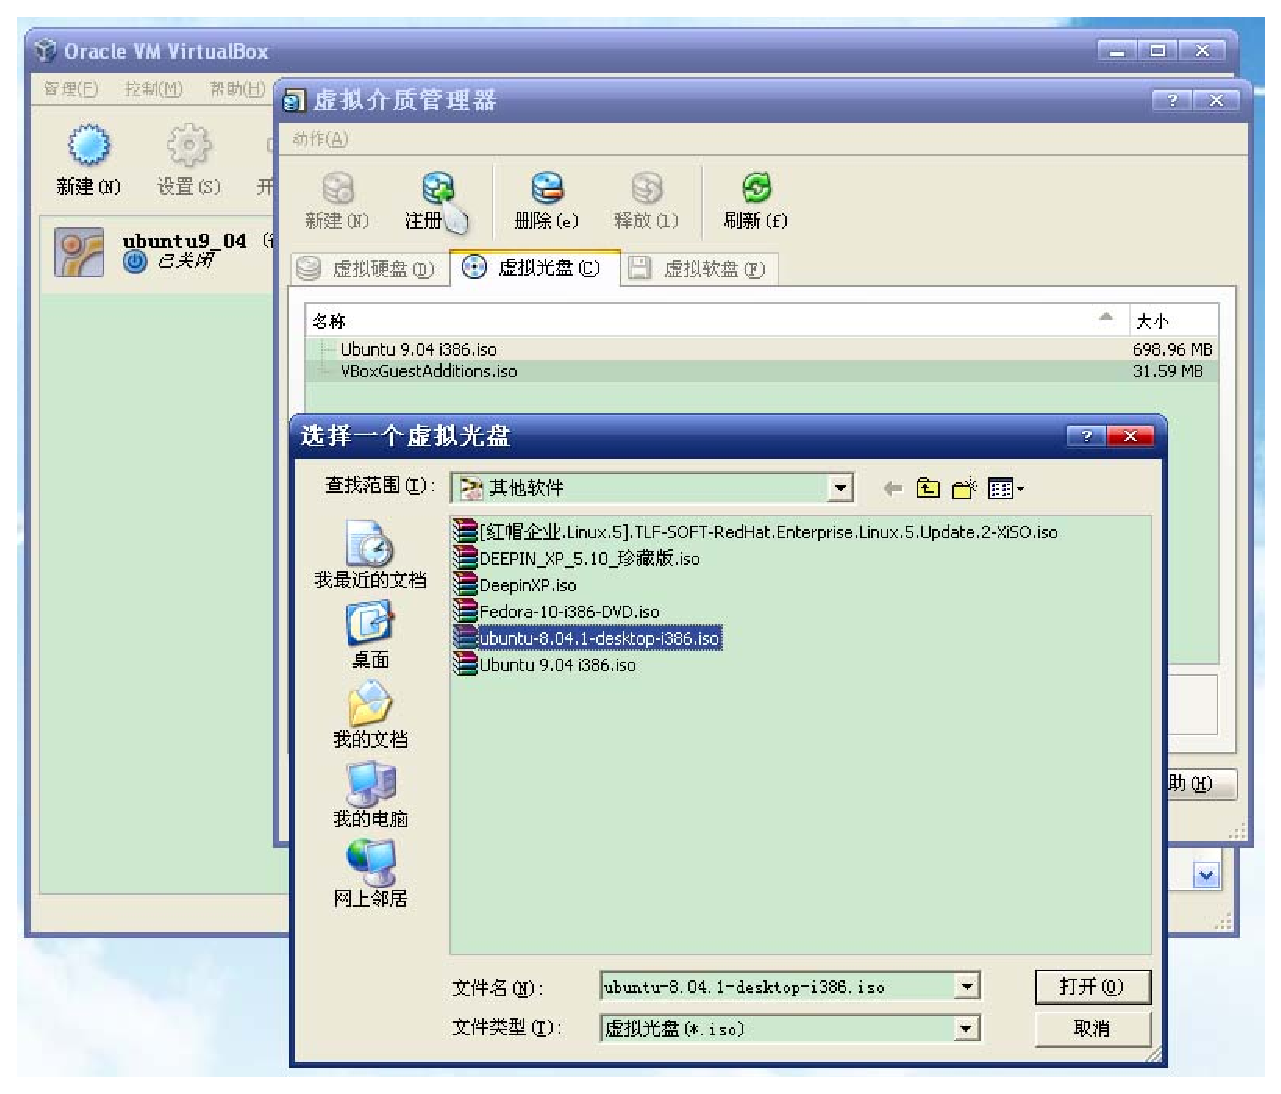
\includegraphics[width=0.8\textwidth,scale=0.8]{pic/f_vb_setting_iso_register.eps}
\caption{设置ISO\label{iso1}}
\end{figure}
\begin{figure}[!bthp]
\centering
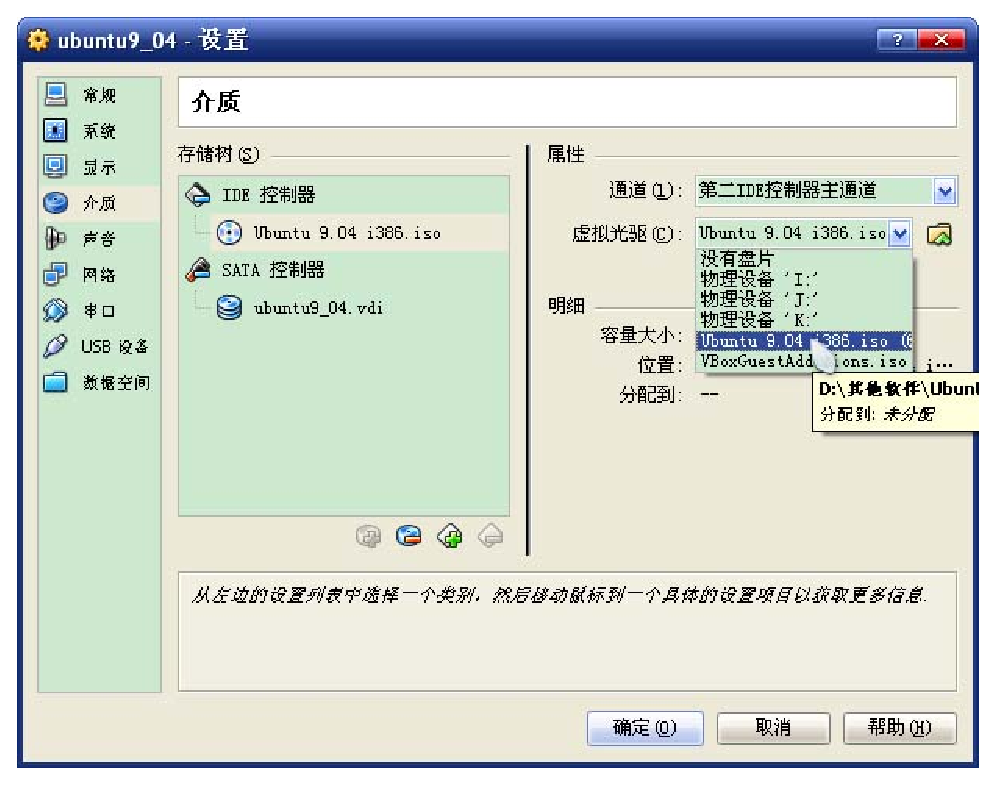
\includegraphics[width=0.8\textwidth,scale=0.8]{pic/f_vb_setting_iso_set.eps}
\caption{设置ISO\label{iso2}}
\end{figure}

之后运行虚拟机,系统就会从ISO进行引导,进而安装Ubuntu系统.过程略.

安装完成后.若宿主机能够访问互联网,则虚拟机也能访问互联网.剩下一个问题就是共享文件夹的设置.在设置之前,需要先安装Virtual Box提供的
增强工具包.在运行虚拟机的界面上选择\fbox{设备-->安装增强功能}.此时在虚拟机的桌面上就会出现一个光盘.打开终端\footnote{Alt+F2调出运行
窗口,输入\fbox{gnome-terminal}回车即可调出终端}.在终端中输入如下命令:
\begin{verse}
\textbf{cd /media/cdrom\\sudo ./VBoxLinuxAdditions-x86.run \#若本地PC是amd64位架构,就运行VBoxLinuxAdditions-amd64.run\\输入管理员密码}
\end{verse}
等待安装过程结束,关闭虚拟机\textit(注意,这里一定要先关闭虚拟机).然后在\fbox{设置}中右侧找到"数据空间",添加一个在宿主机上已经存在的文件夹作为共享目的地.如图\ref{f_sf}所示.
启动虚拟机,终端中输入如下命令:
\begin{verse}
\textbf{mkdir -p /home/<你的用户名>/Desktop/VBS \#在虚拟机中创建一个文件夹\\sudo mount -t vbox <宿主机中共享文件夹名称> 
/home/<你的用户名>/Desktop/VBS}
\end{verse}
经过这番设置后,共享文件夹就设置成功了.
\begin{figure}[!bthp]
\centering
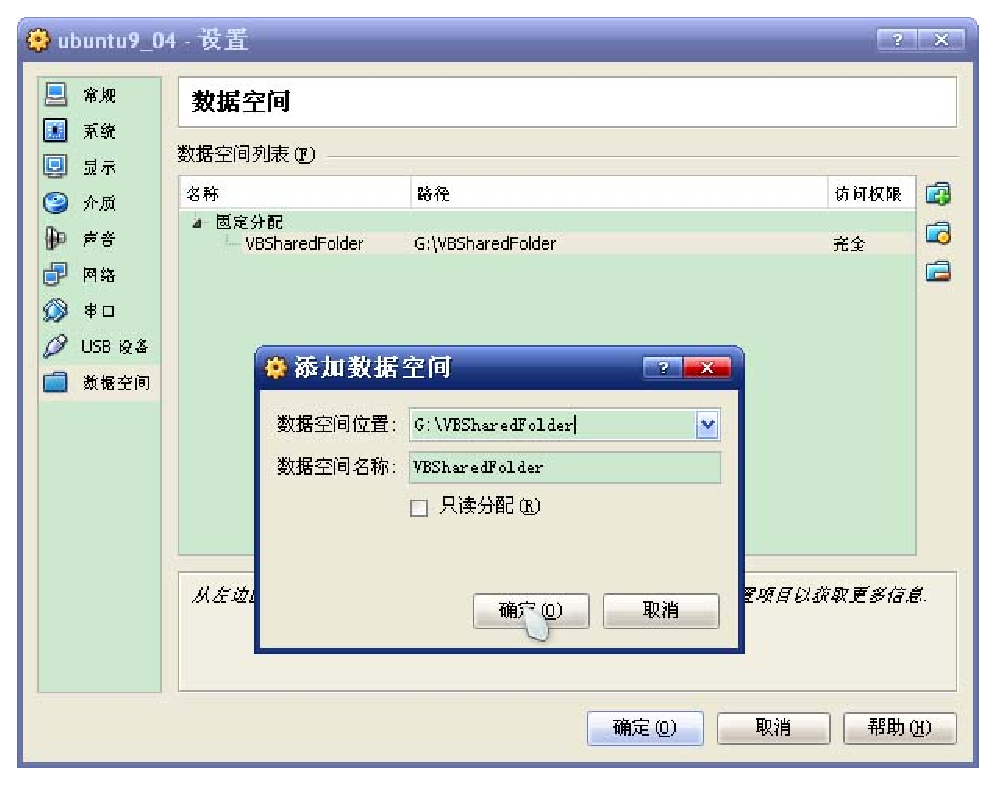
\includegraphics[width=0.8\textwidth,scale=0.8]{pic/f_vb_setting_sf.eps}
\caption{共享空间设置\label{f_sf}}
\end{figure}
\subsubsection{内核开发包安装设置}
\end{document}

